\documentclass[blue,uncompressed]{beamer}
\usepackage{tikz}
\usepackage{graphicx}
%\usepackage{listingsutf8}
\usepackage{listings}
\usepackage[spanish]{babel}
\usepackage[utf8]{inputenc}
\usepackage{multirow}
\pdfinfo
{
  /Title       (BulletPoint. Tecnología beacon en entornos universitarios.)
  /Creator     (Laura Padrón Jorge)
  /Author      (Laura Padrón Jorge)
  /Subject     (Trabajo de Fin de Grado)
}
%%%%%%%%%%%%%%%%%%%%%%%%%%%%%%%%%%%%%%%%%%%%%%%%%%%%%%%%%%%%%%%%%%%%%%%%%%%%%%%%%%%%%%%%%%%%
% Definiendo colores para los listados de código fuente - Univ. Deusto
\definecolor{violet}{rgb}{0.5,0,0.5}
\definecolor{navy}{rgb}{0,0,0.5}
\definecolor{hellgelb}{rgb}{1,1,0.8}
\definecolor{colKeys}{rgb}{0,0,53}           %%% Todo : check color for keys
\definecolor{colIdentifier}{rgb}{0,0,0}
\definecolor{colComments}{rgb}{1,0,0}
\definecolor{colString}{rgb}{0,0.5,0}
\definecolor{lightlightgray}{rgb}{204,204,204}

\definecolor{marron}       {rgb}{0.496, 0.203, 0.152}
\definecolor{verde-claro}  {rgb}{0.625, 0.734, 0.199}
\definecolor{oscuro}       {rgb}{0.187, 0.141, 0.285}
\definecolor{gris}     	   {rgb}{0.500, 0.500, 0.500}
\definecolor{bgd-listings} {rgb}{0.999, 0.999, 0.900}
\definecolor{gray97}{gray}{.97}
\definecolor{gray75}{gray}{.75}
\definecolor{gray45}{gray}{.45}
\definecolor{gray}{gray}{.45}
%%%%%%%%%%%%%%%%%%%%%%%%%%%%%%%%%%%%%%%%%%%%%%%%%%%%%%%%%%%%%%%%%%%%%%%%%%%%%%%%%%%%%%%%%%%%
\lstloadlanguages{Java}
\lstloadlanguages{XML}
\lstset{
	float=hbp,
		language = Java,
			morekeywords={hicuda,global,alloc,shape,kernel,thread,loop_partition,tblock,over_tblock,over_thread,kernel_end,copyout,free,data,region,task,input,inout,output,pragma,omp,parallel,reduction,private,shared,target,device,copy_in,copy_out,acc,kernels,loop,copyin,copy,pcopy,pcopyin,collapse,gang,worker,independent,firstprivate,endfor,in},
				%\emph      ={omp,parallel,reduction,private,shared},
				xleftmargin=5.0ex,    % Margen izq. para que los números de línea se vean
				emphstyle=\textbf,
        basicstyle=\ttfamily\scriptsize,
        identifierstyle=\color{colIdentifier},
        keywordstyle=\color{colKeys},
        stringstyle=\color{colString},
        commentstyle=\color[rgb]{0.133,0.545,0.133},
        columns=flexible,
        tabsize=4,
        frame=single,
        extendedchars=true,
        showspaces=false,
        showstringspaces=false,
        numbers=left,
        numberstyle=\tiny,
        breaklines=true,
        backgroundcolor=\color{lightlightgray},
        breakautoindent=true,
        captionpos=b
        morecomment=[l][\color{colKeys}]{\#}
}
%%%%%%%%%%%%%%%%%%%%%%%%%%%%%%%%%%%%%%%%%%%%%%%%%%%%%%%%%%%%%%%%%%%%%%%%%%%%%%%%%%%%%%%%%%%%
\mode<handout>
{
	\usepackage{pgfpages}
	\pgfpagesuselayout{2 on 1}[a4paper,border shrink=5mm]
	\setbeamercolor{background canvas}{bg=black!0}
	\setbeameroption{show notes}
}

\mode<presentation>
{
	\usetheme{Madrid}
	\usecolortheme{ull}
	\setbeamercovered{transparent}
	%\logo{  % Logo ULL en esquina inferior derecha
	%    \includegraphics[width=.25\textwidth]{FIGURES/logoull-oficial.png}
	%}
}
%%%%%%%%%%%%%%%%%%%%%%%%%%%%%%%%%%%%%%%%%%%%%%%%%%%%%%%%%%%%%%%%%%%%%%%%%%%%%%%%%%%%%%%%%%%%
\AtBeginSection[]
{
	\begin{frame}<beamer>
		\frametitle{Outline}
		\tableofcontents[currentsection,currentsubsection]
	\end{frame}
}
%%%%%%%%%%%%%%%%%%%%%%%%%%%%%%%%%%%%%%%%%%%%%%%%%%%%%%%%%%%%%%%%%%%%%%%%%%%%%%%%%%%%%%%%%%%%
\title{\textbf{BulletPoint}}
\subtitle{Tecnología beacon en entornos universitarios}
\author[Laura Padrón Jorge]
{
	\textbf{Laura Padrón Jorge}
	%\alert{Francisco~de Sande} \\
	%\url{fsande@ull.es}
}
\institute[ULL]

\date[Trabajo de Fin de Grado]{\textsc{Trabajo de Fin de Grado}     \\
                           La Laguna, 15 de Julio, 2016}
\subject{TFG}

\AtBeginSection[]
{
	\frame<handout:0>
		{
			\frametitle{Índice}
			\tableofcontents[current]
		}
}
%%%%%%%%%%%%%%%%%%%%%%%%%%%%%%%%%%%%%%%%%%%%%%%%%%%%%%%%%%%%%%%%%%%%%%%%%%%%%%%%%%%%%%%%%%%%
\newcommand{\BulletPoint}{\texttt{BulletPoint{}}}

\setbeamerfont{title}{size=\Large,shape=\sffamily}
\setbeamerfont{author}{size=\small,shape=\sffamily}
\setbeamerfont{institute}{size=\scriptsize,shape=\sffamily}
\setbeamerfont{date}{size=\scriptsize,shape=\sffamily}
%%%%%%%%%%%%%%%%%%%%%%%% Title Page %%%%%%%%%%%%%%%%%%%%%%%%%%%%%%%%%%%%%%%%%%%%%%%%%%%%%%%%%%%%%%%%%%%%
\defbeamertemplate*{title page}{AGH}[1][]
{
  \vbox{}
  %\vspace*{2.3cm}
  \vfill 
\includegraphics[width=0.15\linewidth]{Images/logos/logo_vertical}
    \vfill
  %\hspace*{1.8cm}
  \begin{columns}
    \begin{column}{0.6\textwidth}
      \begin{beamercolorbox}[sep=8pt,#1]{title}
	\centering{\usebeamerfont{title}\inserttitle\par}
	\ifx\insertsubtitle\@empty%
	\else%
	  \vskip0.25em%
	  {\usebeamerfont{subtitle}\usebeamercolor[fg]{subtitle}\insertsubtitle\par}%
	\fi%
	
      \end{beamercolorbox}%
      \vskip1em\par
      \hspace*{2.35cm}
      \begin{beamercolorbox}[sep=8pt,#1]{author}
	\usebeamerfont{author}\insertauthor
      \end{beamercolorbox}
      \vskip1em\par
      \hspace*{2.35cm}
      \begin{beamercolorbox}[sep=8pt,#1]{institute}
	\usebeamerfont{institute}\insertinstitute
      \end{beamercolorbox}
      \hspace*{2.35cm}
      \begin{beamercolorbox}[sep=8pt,#1]{date}
	\usebeamerfont{date}\insertdate
      \end{beamercolorbox}\vskip0.5em
    \end{column}
    
    \begin{column}{0.4\textwidth}
      \hfill 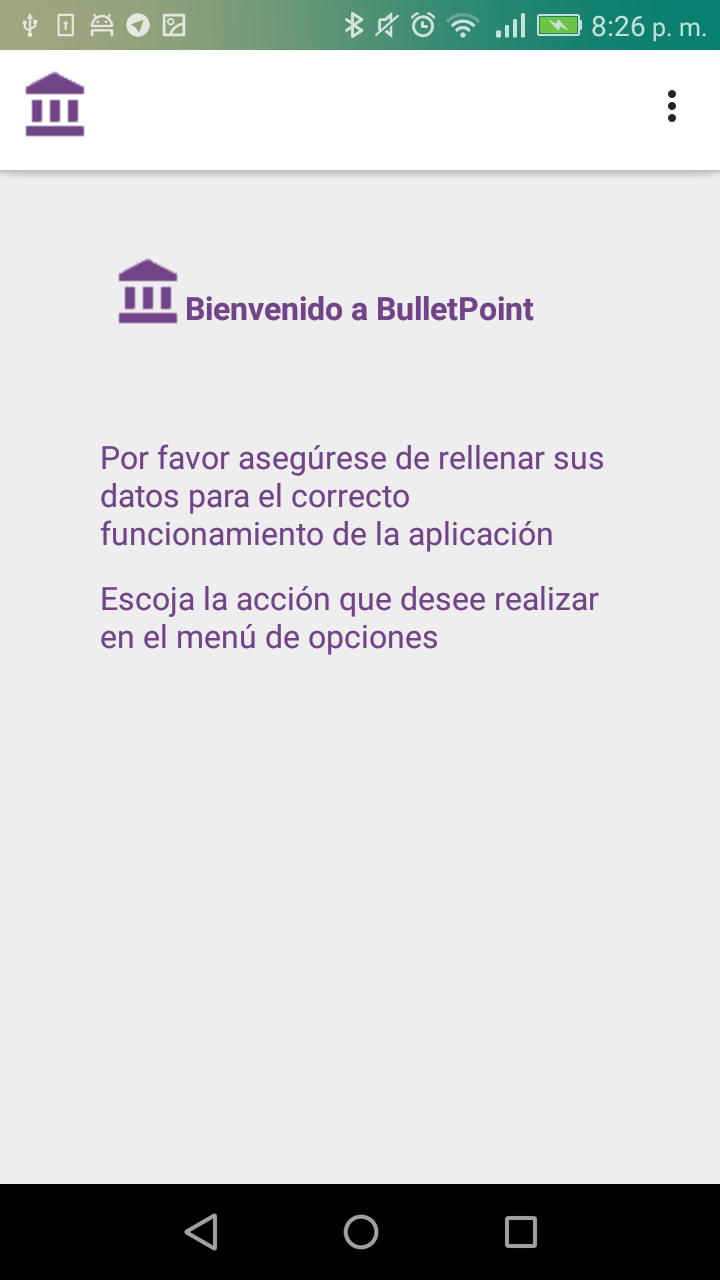
\includegraphics[width=0.8\linewidth]{Images/App/menuPrincipal.png}
    \end{column}
  \end{columns}
    %\hfill \includegraphics[width=0.2\linewidth]{Images/varios/MainActivity.png}
    %{\usebeamercolor[fg]{titlegraphic}\inserttitlegraphic\par}
	%	\vfill \includegraphics[width=0.3\linewidth]{FIGURES/logos/nwo}
	%	\hfill \includegraphics[width=0.17\linewidth]{FIGURES/logos/stw}
	%	\hfill \includegraphics[width=0.2\linewidth]{FIGURES/logos/ipn.jpg}
  %\vfill
}
%%%%%%%%%%%%%%%%%%%%%%%%%%%%%%%%%%%%%%%%%%%%%%%%%%%%%%%%%%%%%%%%%%%%%%%%%%%%%%%%%%%%%%%%%%%%
% Slide numbers. 
%\expandafter\def\expandafter\insertshorttitle\expandafter{%
%  \insertshorttitle\hfill%
%  \insertframenumber\,/\,\inserttotalframenumber
%}
%%%%%%%%%%%%%%%%%%%%%%%%%%%%%%%%%%%%%%%%%%%%%%%%%%%%%%%%%%%%%%%%%%%%%%%%%%%%%%%%%%%%%%%%%%%%
\begin{document}
	%\frame{\titlepage}
	\begin{frame}[plain]
	\titlepage
	\end{frame}

	\frame{\frametitle{Índice}\tableofcontents}
		\section{Introducción}
			\begin{frame}
    \frametitle{Introducción}
    %\block{Objetivo del TFG}
    \begin{itemize}
	\item \textbf{Tutor Trabajo Fin de Grado:} Francisco de Sande González
        \item \textbf{Línea de trabajo del proyecto:} Programación de aplicaciones interactivas en {\it Android}.
    \end{itemize}
    %\endblock{}
        {\usebeamercolor[fg]{titlegraphic}\inserttitlegraphic\par}
		\vfill 
\includegraphics[width=0.2\linewidth]{Images/logos/aruba_networks}
		\hfill %
		
\includegraphics[width=0.2\linewidth]{Images/logos/android_logo}
		\hfill 
\includegraphics[width=0.35\linewidth]{Images/logos/couchbase_logo}
\end{frame}
% -------------------------------------------------------------------------
\begin{frame}
	\frametitle{Introducción}
	\block{Objetivos}
		\begin{itemize}
			\item Desarrollo de un proyecto de Ingeniería.
			\item Programación de aplicaciones en Android.
			\item Realidad aumentada.
			\item Plataforma como servicio (PaaS).
			\item Repositorio online.
			\item Creación de una memoria técnica.
			\item \textit{LaTeX}.
			\item Guia de uso de estas tecnologías en el proyecto.
		\end{itemize}
	\endblock{}	
\end{frame}  
% -------------------------------------------------------------------------
		\section{Herramientas y Tecnologías utilizadas}
			\begin{frame}
	\frametitle{Herramientas y Tecnologías utilizadas}
	\block{ Android Studio}
		\begin{itemize}
			\item Entorno de desarrollo integrado.
			\item Gradle.
			\item Sistema de depuración sencillo e intuitivo.
		\end{itemize}
	\endblock{}
\end{frame}

%------------------------------------------------------------------
\begin{frame}
	\frametitle{Herramientas y Tecnologías utilizadas}
	\block{\it Realidad Aumentada (RA)}
		\begin{itemize}
			\item {\it ¿Qué es la RA?}.
			\item {\it ¿Cómo funciona esta tecnología?}.
			\item {\it ¿Qué tipos de Realidad Aumentada existen?}.
			\item {\it ¿Diferencias entre la Realidad Aumentada y la Realidad Virtual (RV)?}.
			\item {\it ¿Qué es la Realidad Mixta?}.
			\item {\it ¿Qué futuro le espera a la RA?}.
			\item {\it Integración de la RA en Android Studio}.
		\end{itemize}
	\endblock{}
\end{frame}

%------------------------------------------------------------------

\begin{frame}
	\frametitle{Herramientas y Tecnologías utilizadas}
		\block{\it ¿Qué es la realidad aumentada?}
		\begin{itemize}
			\item Permite expandir la información del mundo físico.
			\item Se encuentra en su mejor momento.
			\item Aplicaciones para todos los ámbitos. 
		\end{itemize}
		\endblock{}

		\begin{center}
			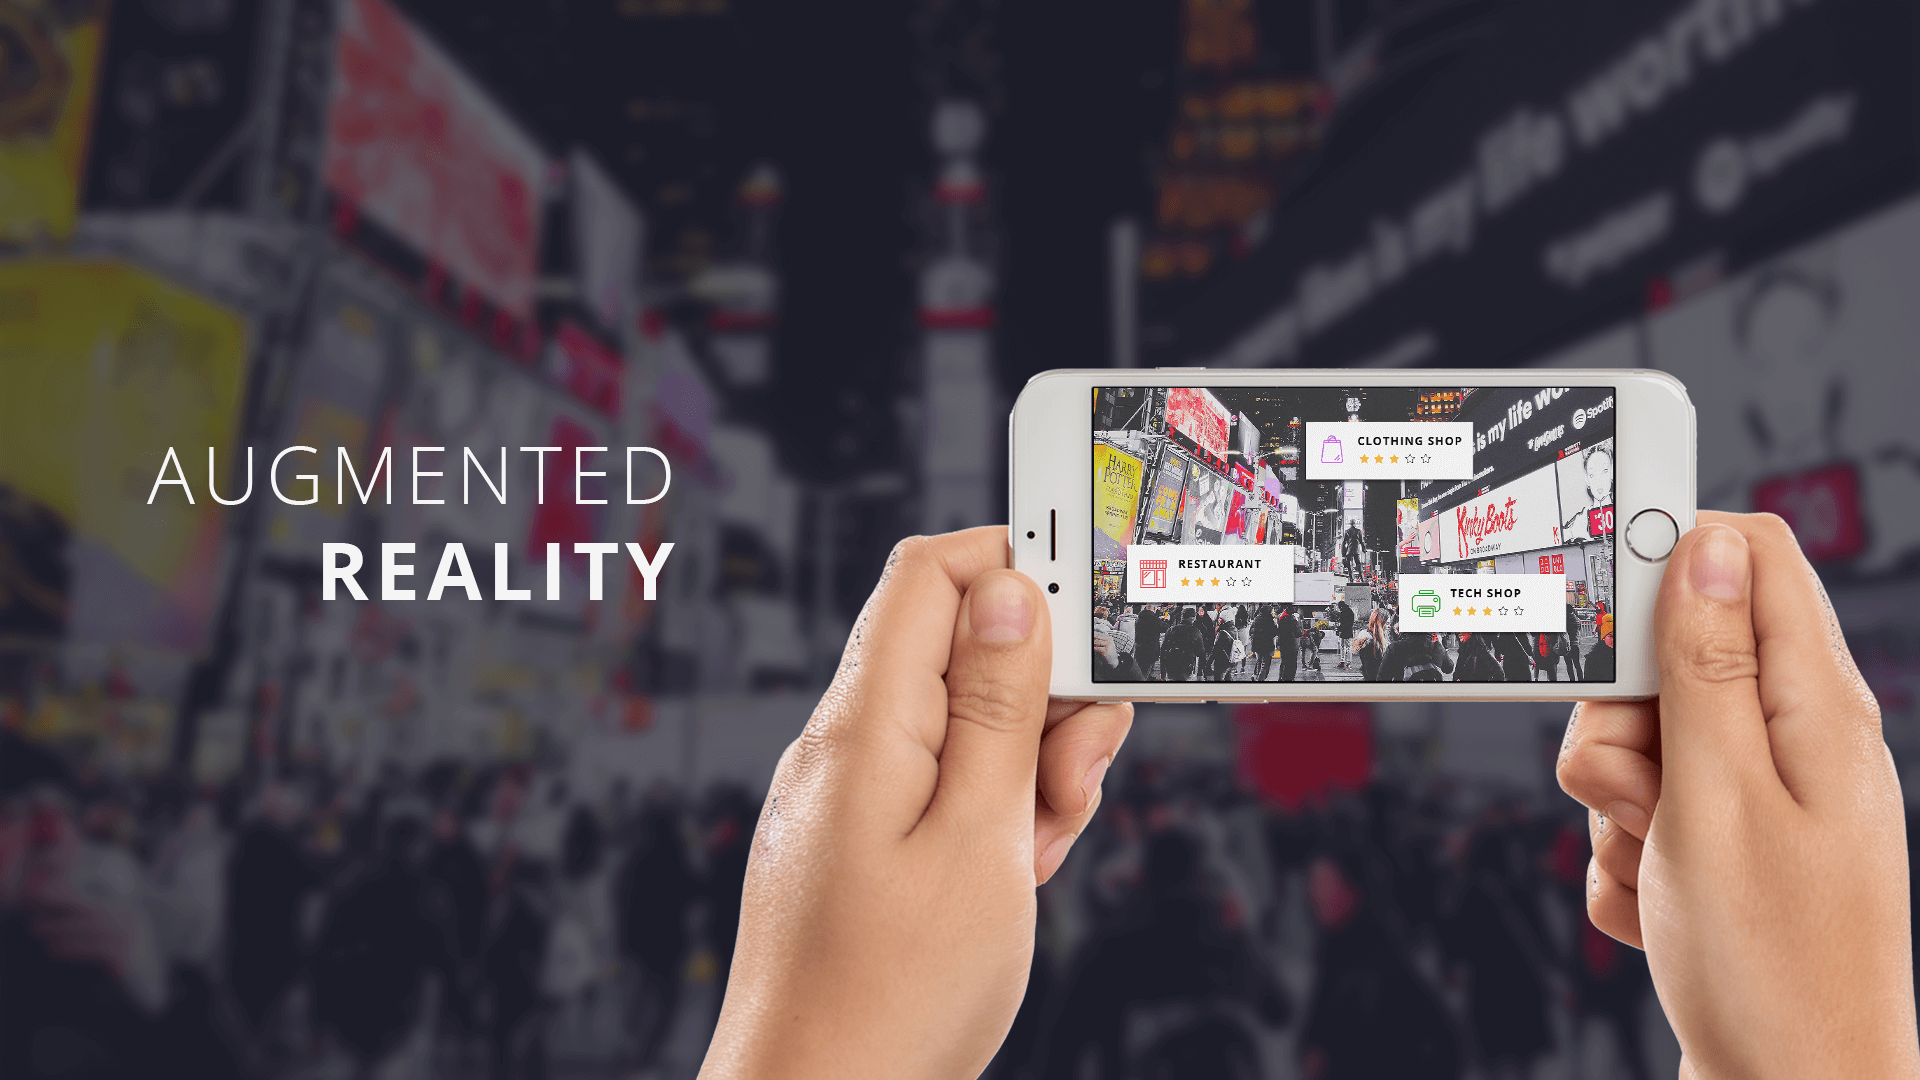
\includegraphics[width=0.7\linewidth]{Images/ar3}
		\end{center}
	
\end{frame}

%------------------------------------------------------------------
\begin{frame}
	\frametitle{Herramientas y Tecnologías utilizadas}
		\block{\it ¿Cómo funciona esta tecnología?}
			Componentes necesarios para la tecnología de RA:
			\begin{itemize}
				\item {Dispositivo de visualización.}
				\item {Sistema de computación.}
				\item {Sensores: GPS, WIFI, Bluetooth, acelerómetro, giroscopio, cámara, etc.}
				\item {Software de RA.}
			\end{itemize}
		\endblock{}

		\begin{center}
			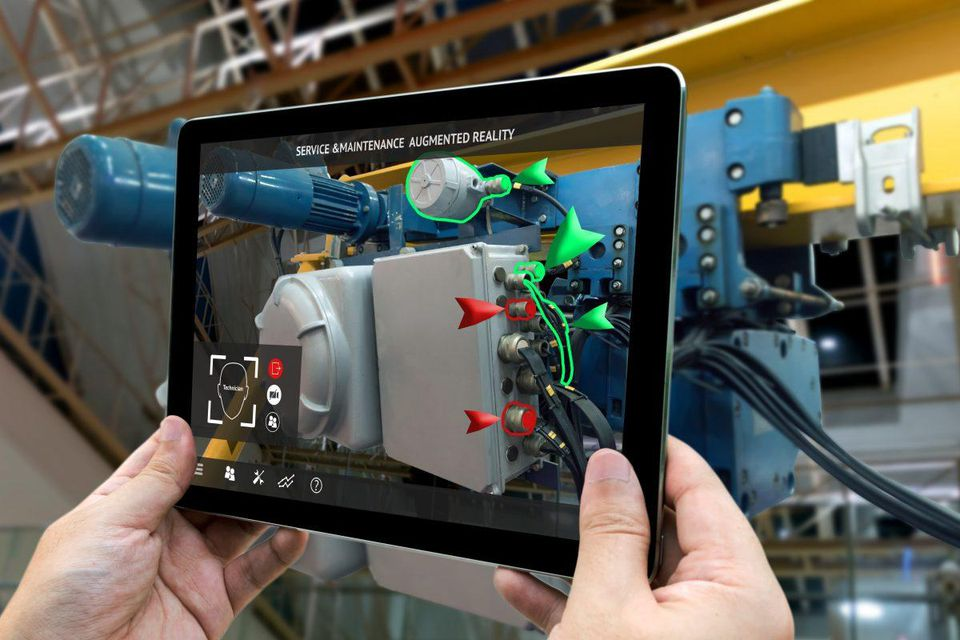
\includegraphics[width=0.43\linewidth]{Images/ar1}
		\end{center}
\end{frame}
		


\begin{frame}
	\frametitle{Herramientas y Tecnologías utilizadas}
	\begin{columns}
			\begin{column}{0.45\textwidth}
				\block{\it ¿Qué tipos de RA existen?}
					Existen distintos tipos de RA:
					\begin{itemize}
						\item {Marker-based AR.}
						\item {Markerless AR.}
						\item {Pojection-based AR.}
						\item {Superimposition-based AR.}
					\end{itemize}
				\endblock{}
			\end{column}
			\begin{column}{0.55\textwidth}
				\vfill 
					\begin{center}
						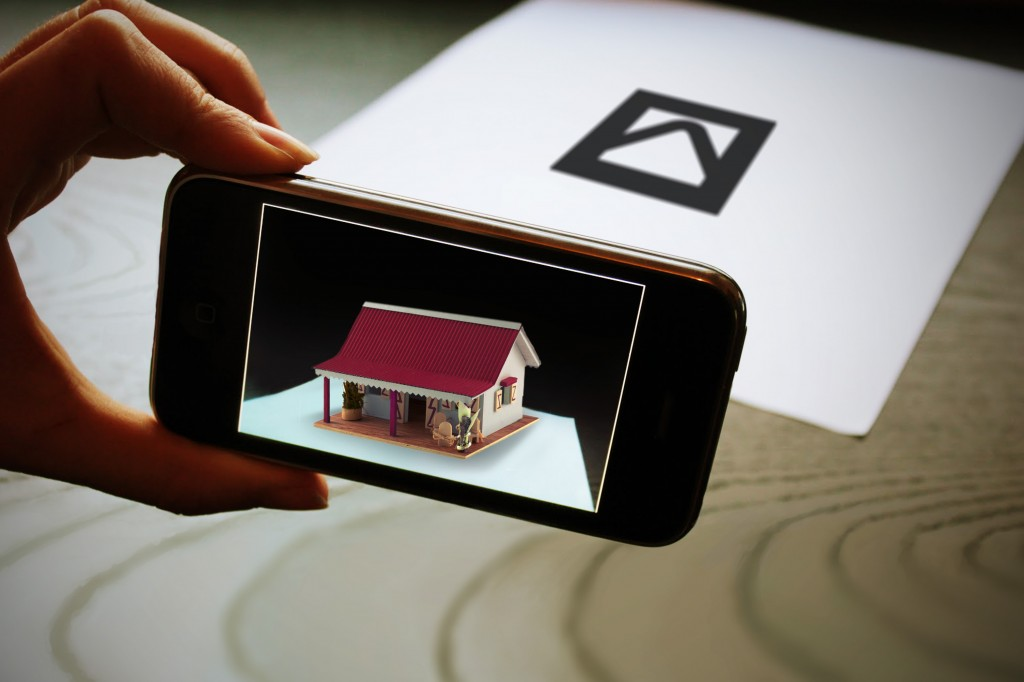
\includegraphics[width=0.95\linewidth]{Images/marker-ar}
					\end{center}
			\end{column}
	\end{columns}
\end{frame}

%------------------------------------------------------------------

\begin{frame}
	\frametitle{Herramientas y Tecnologías utilizadas}
		\block{\it ¿Diferencias entre la Realidad Aumentada y la Realidad Virtual (RV)?}
			\begin{itemize}
				\item {En la actualidad se encuentra más avanzada que la RA.}
				\item {Muestra al usuario un entorno de escenas y objetos de aperiencia real.}
				\item {Dispone de distintos mecanismos de interacción.}
				\item {Aleja al usuario del entorno real.}
			\end{itemize}
		\endblock{}
			\begin{center}
				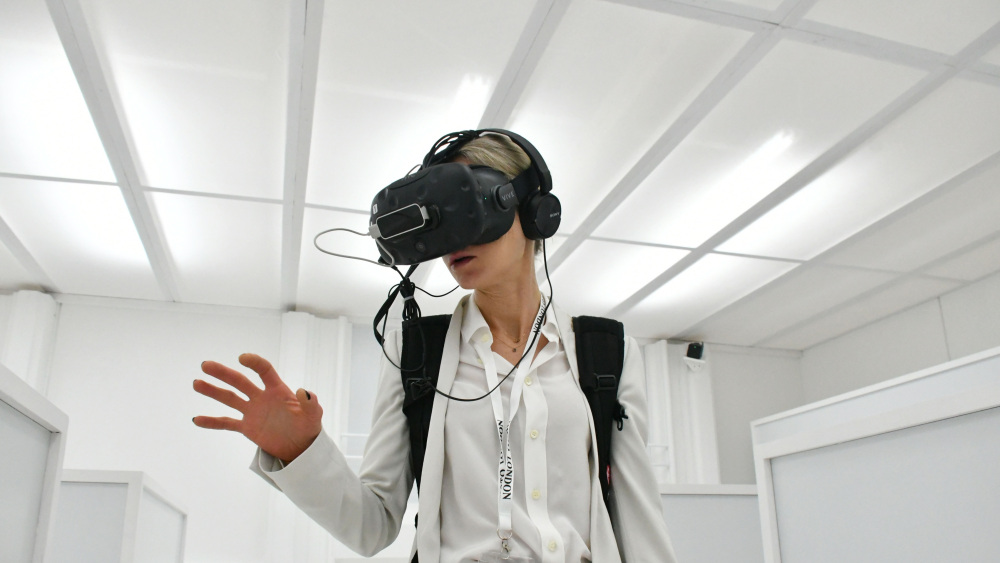
\includegraphics[width=0.50\linewidth]{Images/vr1}
			\end{center}
\end{frame}

%--------------------------------------------------------------------


\begin{frame}
	\frametitle{Herramientas y Tecnologías utilizadas}
		\block{\it ¿Qué es la Realidad Mixta?}
			\begin{itemize}
				\item {Es la union de la RA con la RV}.
				\item {Consiste en llevar el mundo real al mundo virtual.}
				\item {Requiere de mayor capacidad de procesamiento que la RA.}
			\end{itemize}
		\endblock{}
		\vfill 
			\begin{center}
				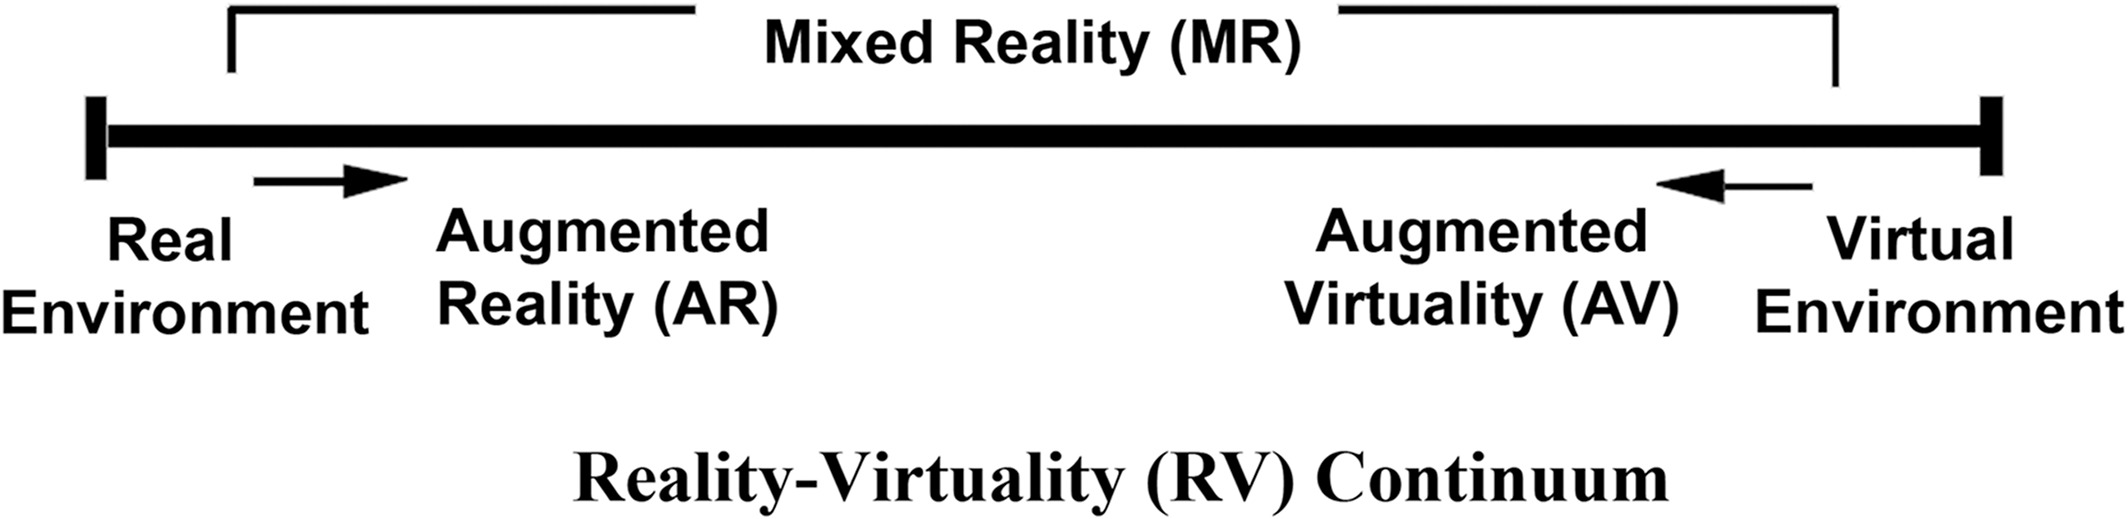
\includegraphics[width=0.8\linewidth]{Images/realidamixta}
			\end{center}
\end{frame}


\begin{frame}
	\frametitle{Herramientas y Tecnologías utilizadas}
	\block{\it ¿Qué futuro le espera a la Realidad Aumentada?}
		Los usos de la RA se acercan a todos los sectores:
		\begin{itemize}
			\item {Educación}.
			\item {Videojuegos.}
			\item {Industria.}
			\item {Turismo.}
			\item {Medicina.}
		\end{itemize}

	\endblock{}
\end{frame}



\begin{frame}
	\frametitle{Herramientas y Tecnologías utilizadas}
	\block{\it  Integración de la Realidad Aumentada en Android Studio}
		\begin{columns}
			\begin{column}{0.3\textwidth}
				\begin{center}					
					Vuforia 
				\end{center}
				\vspace{3mm}
				\vfill 
					\begin{center}
						
\includegraphics[width=0.8\linewidth]{Images/vuforia}
					\end{center}
			\end{column}
			\begin{column}{0.3\textwidth}
				\begin{center}
				Kudan AR SDK
				\end{center}
				\vspace{3mm}
				\vfill 
					\begin{center}
						
\includegraphics[width=0.8\linewidth]{Images/kudan}
					\end{center}
			\end{column}
			\begin{column}{0.3\textwidth}
				\begin{center}
					MaxST SDK
				\end{center}
				\vspace{3mm}
				\vfill 
					\begin{center}
						
\includegraphics[width=0.5\linewidth]{Images/maxst}
					\end{center}
			\end{column}
		\end{columns}
	\endblock{}
\end{frame}

\begin{frame}
	\frametitle{Herramientas y Tecnologías utilizadas}
		\block{\it Node.js}
			\begin{itemize}
				\item {¿Qué es?}.
				\item {¿Cómo funciona?}.
				\item {¿Por qué se ha decidido utilizar esta tecnología?}.
			\end{itemize}
		\endblock{}
		\vfill 
			\begin{center}
				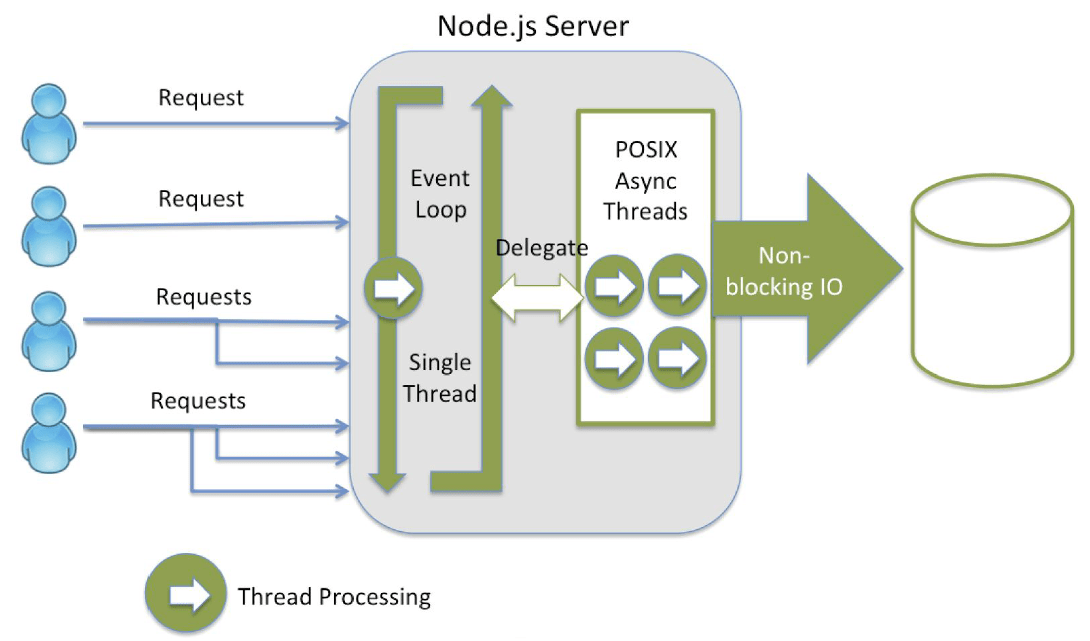
\includegraphics[width=0.72\linewidth]{Images/nodejsEx}
			\end{center}
\end{frame}

\begin{frame}
	\frametitle{Herramientas y Tecnologías utilizadas}
		\block{\it MongoDB}
			\begin{itemize}
				\item {Base de datos NoSQL}.
				\item {De esquema libre}.
				\item {¿Porqué se ha decidido utilizar MongoDB?}.
			\end{itemize}
		\endblock{}
		\vfill 
		\begin{center}
			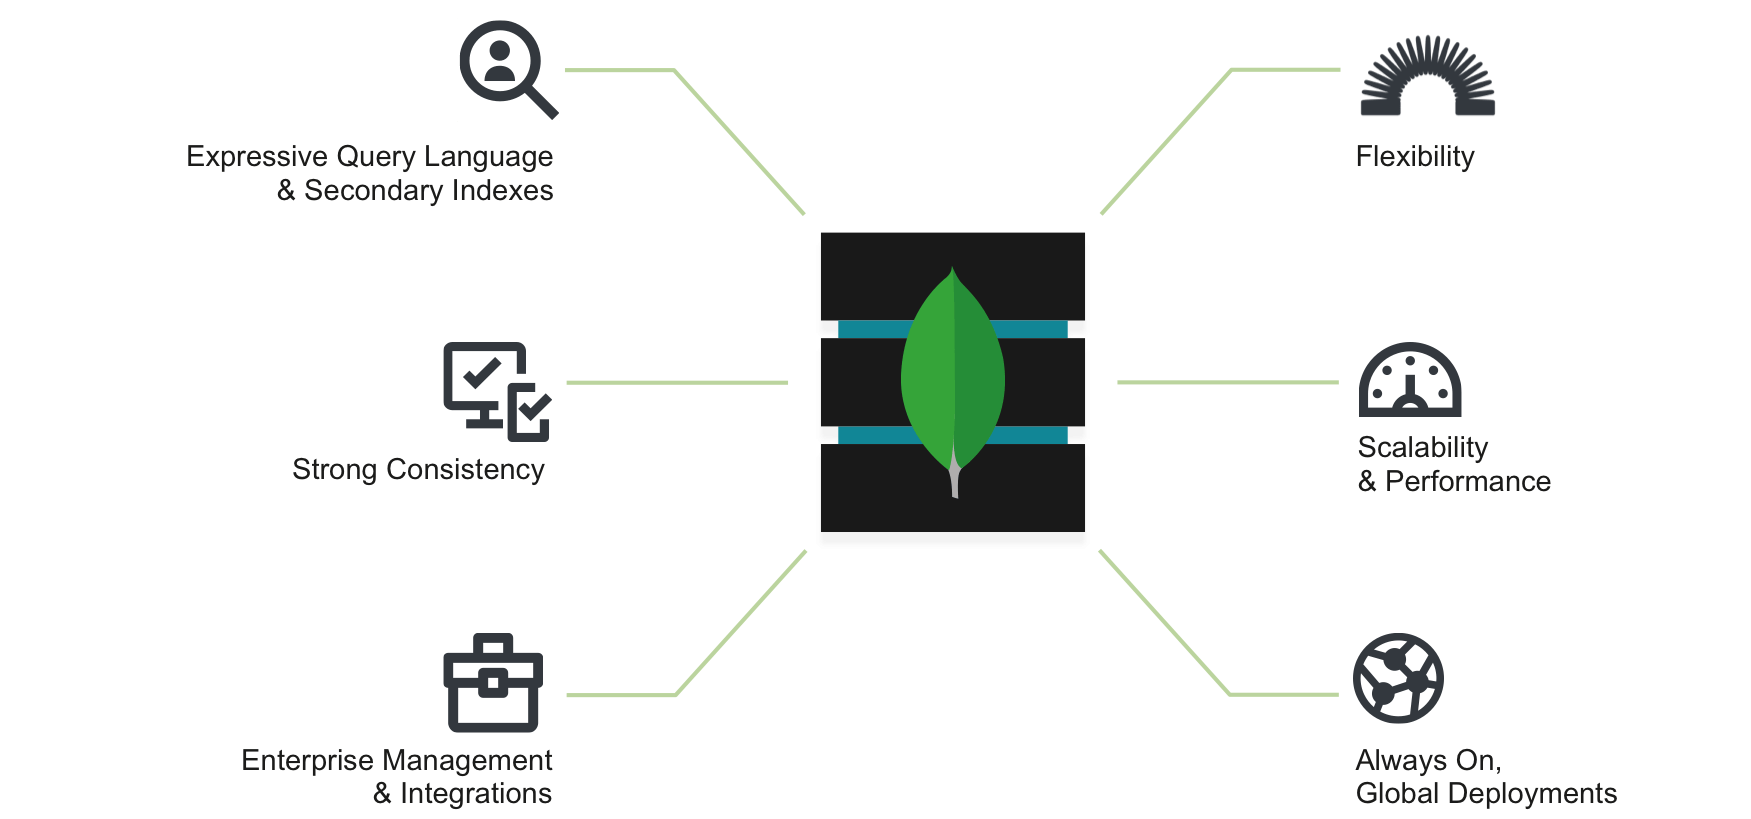
\includegraphics[width=0.88\linewidth]{Images/mongodb-architecture}
		\end{center}
\end{frame}

\begin{frame}
	\frametitle{Herramientas y Tecnologías utilizadas}
	\begin{columns}
			\begin{column}{0.6\textwidth}
				\block{\it Heroku}
					\begin{itemize}
						\item {Plataforma como servicio de computación (PaaS) en la nube}.
						\item {Soporta distintos lenguajes de programación}.
						\item {Ejecuta las aplicaciones en ``dynos''.}
						\item {Servidor de \ULLAR{}}.
					\end{itemize}
				\endblock{}
			\end{column}
			\begin{column}{0.4\textwidth}
				\vfill 
					\begin{center}
						
\includegraphics[width=0.9\linewidth]{Images/heroku}
					\end{center}
			\end{column}
	\end{columns}
\end{frame}

\begin{frame}
	\frametitle{Herramientas y Tecnologías utilizadas}
	\begin{columns}
			\begin{column}{0.6\textwidth}
				\block{\it mLab}
					\begin{itemize}
						\item {Servicio de base de datos como servicio en la nube}
						\item {Ofrece bases de datos MongoDB}.
						\item {Ejecuta sus máquinas en proveedores de servicios en la nube como AWS, Azure y Google Cloud.}
						\item {Base de datos de \ULLAR{}.}
					\end{itemize}
				\endblock{}
			\end{column}
			\begin{column}{0.4\textwidth}
				\vfill 
					\begin{center}
						
\includegraphics[width=0.8\linewidth]{Images/mlab}
					\end{center}
			\end{column}
	\end{columns}
\end{frame}

\begin{frame}
	\frametitle{Herramientas y Tecnologías utilizadas}
		\block{\it Google Maps}
			\begin{itemize}
				\item {API de Google Maps.}
				\item {Permite integrar los mapas de Google Maps en una aplicación Android.}
				\item {Permite:}
				\begin{itemize}
					\item {Creación de marcadores, polígonos y superposiciones.}
					\item {Cambiar la vista del mapa.}
					\item {La posibilidad de elegir el tipo de mapa}
				\end{itemize}
			\end{itemize}
		\endblock{}
\end{frame}

%--------------------------------------------------------------------

		\section{Beacons en entornos universitarios}
			\begin{frame}
	\frametitle{Beacons en entornos universitarios}
			\block{\it Introducción}
				\begin{itemize}
					\item Posibilidades amplias para apps en entornos universitarios.
					\item Cada universidad intenta tener su propia aplicación siguiendo un patrón similar.
					\item Estas aplicaciones se centran en ofrecer servicios propios.
				\end{itemize}
			\endblock{}
\end{frame}

%------------------------------------------------------------------

\begin{frame}
	\frametitle{Beacons en entornos universitarios}
		\begin{columns}
			\begin{column}{0.6\textwidth}
				\block{\it Posibles casos de uso en entornos universitarios}
					\begin{itemize}
						\item Actividades interactivas por el campus, jornadas de acogida u otros eventos.
						\item Despacho del profesorado e información.
						\item Control de acceso a instalaciones.
					\end{itemize}
				\endblock{}
			\end{column}
			\begin{column}{0.4\textwidth}
				\vfill 
				\begin{center}
					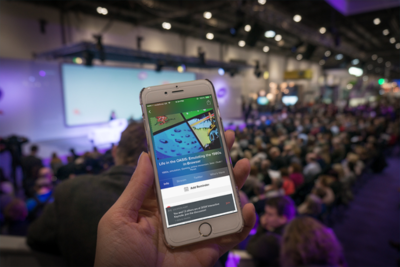
\includegraphics[width=0.9\linewidth]{Images/BeaconEvent}
				\end{center}
			\end{column}		
		\end{columns}
\end{frame}


%---------------------------------------------------------------------

\begin{frame}
	\frametitle{Beacons en entornos universitarios}
		\begin{columns}
			\begin{column}{0.6\textwidth}
				\block{\it Posibles casos de uso en entornos universitarios}
					\begin{itemize}
						\item Biblioteca informativa.
						\item Información y descuentos para usuarios de la app.
						\item Descarga automática de material.
					\end{itemize}
				\endblock{}
			\end{column}
			\begin{column}{0.4\textwidth}
				\vfill 
				\begin{center}
					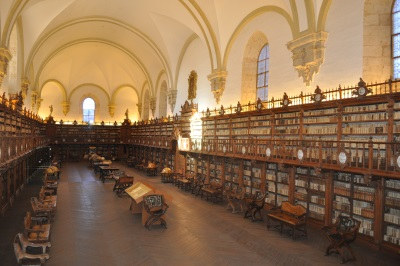
\includegraphics[width=0.9\linewidth]{Images/BibliotecaSalamanca}
				\end{center}
			\end{column}		
		\end{columns}
\end{frame}

		\section{La aplicación \BulletPoint}
			% hablamos de la aplicación

\begin{frame}
	\frametitle{La aplicación \ULLAR{}}
	\block{Requisitos de \ULLAR{}}
	\begin{itemize}
		\item La aplicación se desarrollará para dispositivos con Android. 
		\item Se implementarán técnicas de realidad aumentada basadas en la geolocalización.
		\item El servidor y base de datos de la aplicación estarán alojados en la nube.
	\end{itemize}
	\endblock{}
\end{frame}


\begin{frame}
	\centering{Vídeo demostrativo de la aplicación \ULLAR{}} 
\end{frame}

%--------------------------------------------------------------------

% \begin{frame}
% 	\frametitle{Asociación de MAC a identificador de }
% 	\lstinputlisting{Code/BeaconBusStop.java}
% \end{frame}

%--------------------------------------------------------------------
% Explicación activity y layout
%--------------------------------------------------------------------

% \begin{frame}
% 	\frametitle{Inicio de la aplicación}
% 	\begin{columns}
% 		\begin{column}{0.6\textwidth}
% 			\block{Splash Screen}
% 			\begin{itemize}
% 				\item Logo de \ULLAR{}.
% 				\item Mejor apariencia.
% 				\item Pantalla de carga de la aplicación.
% 			\end{itemize}
% 			\endblock{}
% 		\end{column}
% 		\begin{column}{0.4\textwidth}
% 			\vfill 
% 			\begin{center}
% 				
\includegraphics[width=0.7\linewidth]{Images/splashApp}
% 			\end{center}
% 		\end{column}
% 	\end{columns}
% \end{frame}

%--------------------------------------------------------------------
 

\begin{frame}
	\frametitle{Inicio de la aplicación}
	\begin{columns}
		\begin{column}{0.6\textwidth}
			\block{Ventana de  \textit{Inicio de Sesión}}
			\begin{itemize}
				\item Permitir al usuario identificarse con su cuenta de la ULL.
				\item Uso API de Google.
				\item Integrada en Firebase.
			\end{itemize}
			\endblock{}
		\end{column}
		\begin{column}{0.4\textwidth}
			\vfill 
			\begin{center}
				
\includegraphics[width=0.7\linewidth]{Images/loginApp}
			\end{center}
		\end{column}
	\end{columns}
\end{frame}
  
 
\begin{frame}
	\frametitle{Ventana de  \textit{Inicio de Sesión}}
	\lstinputlisting{Code/login1.java}
\end{frame}


\begin{frame}
	\frametitle{Ventana de  \textit{Inicio de Sesión}}
	\lstinputlisting{Code/login2.java}
\end{frame}
%------------------------------------- -------------------------------

\begin{frame}
	\frametitle{Modo de Realidad Aumentada}
	\begin{columns}
		\begin{column}{0.6\textwidth}
			\block{Ventana de  \textit{Navegación en modo RA}}
			\begin{itemize}
				\item RA basada en geolocalización.
				\item Acceso a los sensores del dispositivo.
				\item Identificación de las instalaciones de la ULL.
				\item Obtencion de las instalaciones.
				\item La clase ARNavigation.java es el activity principal encargado.
			\end{itemize}
			\endblock{}
		\end{column}
		\begin{column}{0.4\textwidth} 
			\vfill 
			\begin{center}
				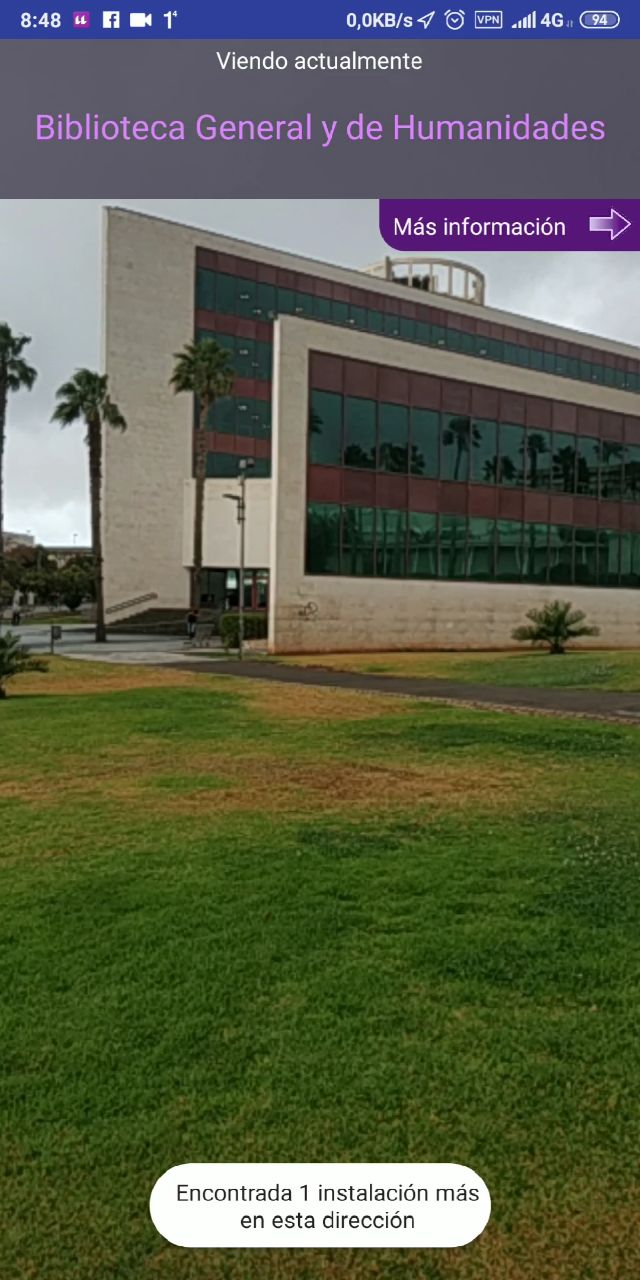
\includegraphics[width=0.7\linewidth]{Images/imagedera}
			\end{center}
		\end{column}
	\end{columns}
\end{frame}

 
\begin{frame}
	\frametitle{Acceso a la ubicación del dispositivo}
	\texttt{AndroidManifest.xml}
	\lstinputlisting{Code/permisosgps.xml}

	\texttt{ARNavigation.java}
	\lstinputlisting{Code/permisosgps2.java}
\end{frame}
%--------------------------------------------------------------------


 
\begin{frame}
	\frametitle{Acceso a la orientación del dispositivo}
	\lstinputlisting{Code/permisosgps3.java}
	\lstinputlisting{Code/permisosgps4.java}
\end{frame}



\begin{frame}
	\frametitle{Acceso a la orientación del dispositivo}
	\block{Orientación de un dispositivo Android}
	\begin{itemize}
		\item Matriz de rotación que Android calcula a partir de magnetómetro y el acelerómetro. 
		\item Se obtiene el valor de brújula magnética del dispositivo.
		\item Permite orientar al dispositivo en el espacio para poder identificar las instalaciones.
	\end{itemize}
	\endblock{}
	\lstinputlisting{Code/brujula.java}
\end{frame}


 


\begin{frame}
	\frametitle{Acceso a la orientación del dispositivo}
		\block{Orientación de un dispositivo Android}
			\begin{itemize}
				\item Android dispone de 3 ejes: x, y, z.
				\item Valor de acimut.
				\item Obtención de la orientación del dispositivo con respecto al norte magnético.
			\end{itemize}
		\endblock{}

		\begin{center} 
			\hspace*{0.5in}
			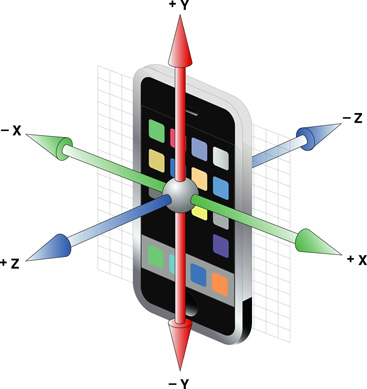
\includegraphics[width=0.3\linewidth]{Images/xyz}
			\hfill
			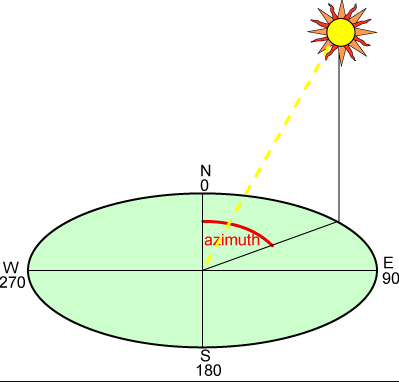
\includegraphics[width=0.3\linewidth]{Images/acimut}
			\hspace*{0.5in}
		\end{center}
\end{frame}		
		

\begin{frame}
	\frametitle{Acceso a la orientación del dispositivo}
	\lstinputlisting{Code/brujula2.java}
\end{frame}


\begin{frame}
	\frametitle{Modo de Realidad Aumentada}
			\block{Modelos encargados de la navegación}
			Clases que intervienen:
			\begin{itemize}
				\item \texttt{ULLSite.java}
				\item \texttt{Navigation.java}
				\item \texttt{Vector2D.java}
			\end{itemize}
			\endblock{}


\end{frame}


\begin{frame}
	\frametitle{Modo de Realidad Aumentada}

			\block{\texttt{ULLSite.java}}
			\begin{itemize}
				\item Almacena la información referente a una instalación de la ULL.
				\item Se crea a partir del objeto JSON contenido en la base de datos.
				\item Contiene los atributos que permiten identificar una instalación.
			\end{itemize}
			\endblock{}

\end{frame}
 
\begin{frame}
	\frametitle{Objeto JSON con la información de una instalación}
	\lstinputlisting{Code/ull_site.json}
\end{frame}

\begin{frame}
	\frametitle{\texttt{ULLSite.java}}
	\lstinputlisting{Code/ULLSite.java}
\end{frame}


\begin{frame}
	\frametitle{\texttt{ULLSite.java}}
			\block{Principales atributos que intervienen en la navegación}
			\begin{itemize}
				\item  ``disToSite''
				\item ``dirToSite''
				\item ``coneValue''
			\end{itemize}
			\endblock{}
			\begin{center} 
				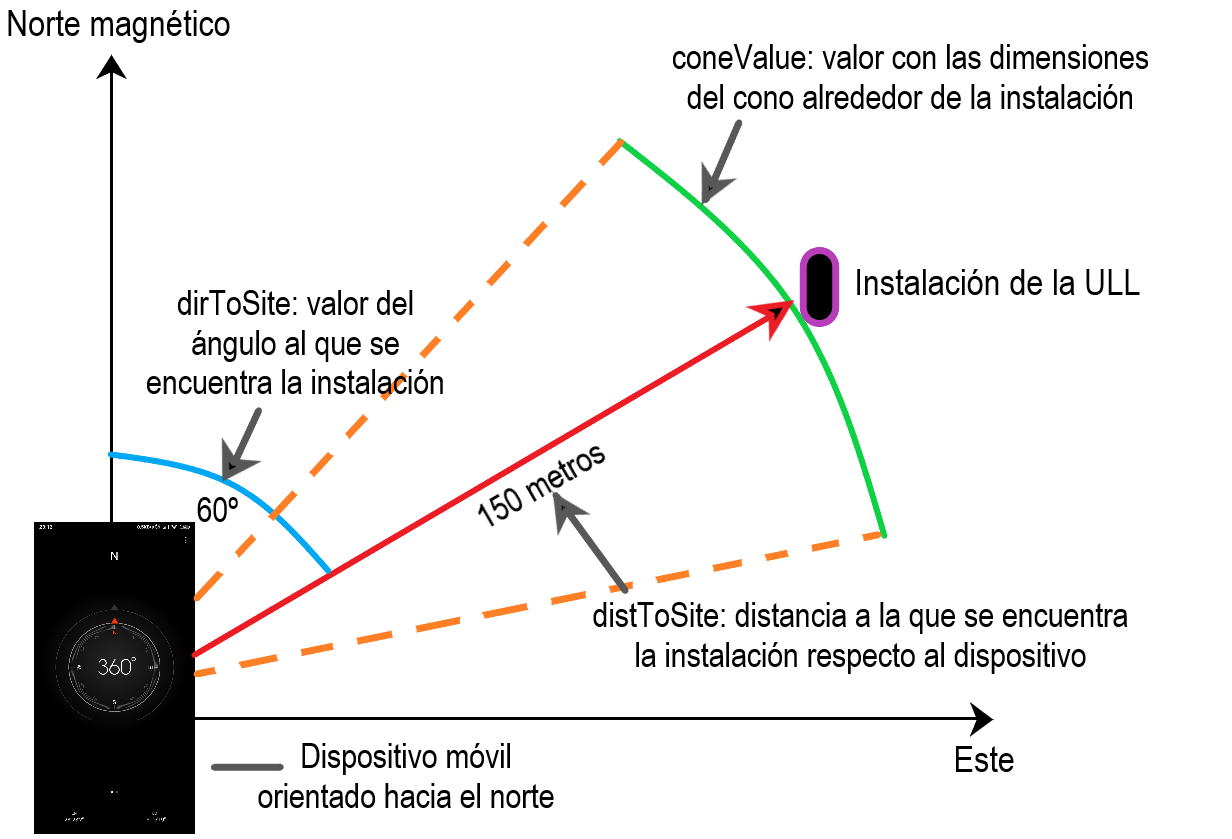
\includegraphics[width=0.65\linewidth]{Images/imagenAR}
			\end{center}
\end{frame}
 
\begin{frame}
	\frametitle{Modelos encargados de la navegación}
			\block{\texttt{Navigation.java}}
			\begin{itemize}
				\item Clase encargada de identificar las instalaciones.
				\item Contiene una lista con todas las instalaciones.
				\item Recibe los datos de los sensores.
				\item Calcula la distancia, dirección y valor de cono para cada instalación.
			\end{itemize}
			\endblock{}
\end{frame}
 
 
\begin{frame}
	\frametitle{Atributos de la clase \texttt{Navigation.java}}
	\lstinputlisting{Code/navigation1.java}
\end{frame}

\begin{frame}
	\frametitle{Métodos de la clase\texttt{Navigation.java}}
	\lstinputlisting{Code/navigation2.java}
\end{frame}

\begin{frame}
	\frametitle{Método calculateCone(double dist)}
	\lstinputlisting{Code/navigation3.java}
\end{frame}
	  
\begin{frame}
	\frametitle{\texttt{Navigation.java}}
	\lstinputlisting{Code/navigation4.java}
	\lstinputlisting{Code/navigation5.java}
\end{frame}

     
\begin{frame}
	\frametitle{whatCanSee(LatLng currentPosAux, double actualDir)}
	\lstinputlisting{Code/navigation6.java}
\end{frame}
\begin{frame}
	\frametitle{whatCanSee(LatLng currentPosAux, double actualDir)}
	\lstinputlisting{Code/navigation7.java}
\end{frame}


\begin{frame}
	\frametitle{Modo de Realidad Aumentada}
			\block{Obtención de la información}
			\begin{itemize}
				\item La información de las instalaciones la provee el servidor que a su vez se comunica con la base de datos.
				\item La clase \texttt{GetData.java} se encarga de conectar con el servidor y manejar la respuesta.
				\item Los radios máximos y minimos con los que identificar las instalaciones están guardados en las Shared Preferences.
			\end{itemize}
			\endblock{}
\end{frame}

\begin{frame}
	\frametitle{\texttt{GetData.java}}
	\lstinputlisting{Code/getdata.java}
\end{frame}

\begin{frame}
	\frametitle{Métodos encargados de la obtención de la información}
	\lstinputlisting{Code/getdata2.java}
	\lstinputlisting{Code/getdata3.java}
\end{frame}

\begin{frame}
	\frametitle{Modo de Realidad Aumentada}
			\block{Visualización}
			\begin{itemize}
				\item El activity ``ARNavigation'' es el encargado de la visualización de la técnica de RA.
				\item Este activity hereda de la clase ``ARActivity'' del SDK de Kudan.
			\end{itemize}
			\endblock{}

\end{frame}

\begin{frame}
	\frametitle{\texttt{arnavigation.xml}}
	\lstinputlisting{Code/visualizacion.xml}
\end{frame}

\begin{frame}
	\frametitle{Fragmentos de \ULLAR{}}
			\block{Fragmentos en Android}
			\begin{itemize}
				\item ¿Qué es un fragmento?
				\item ¿Qué beneficios ofrecen para la aplicación?
				\item Fragmentos de \ULLAR{}:
				\begin{itemize}
					\item MapsFragment.
					\item HomeFragment.
					\item AboutFragment.
				\end{itemize}
			\end{itemize}
			\endblock{}

\end{frame}

    

\begin{frame}
	\frametitle{Fragmentos de \ULLAR{}}
	\begin{columns}
		\begin{column}{0.6\textwidth}
			\block{MapsFragment}
			\begin{itemize}
				\item Nos proporciona un mapa generado por la API de Google Maps.
				\item En este mapa permite:
				\begin{itemize}
					\item Dibujar las instalaciones de la ULL.
					\item Ubicar al dispositivo.
					\item Dibujar dos circunferencias que actuan como rango de aparición de las instalaciones. 
				\end{itemize}
			\end{itemize}
			\endblock{}
		\end{column}
		\begin{column}{0.4\textwidth} 
			\vfill 
			\begin{center}
				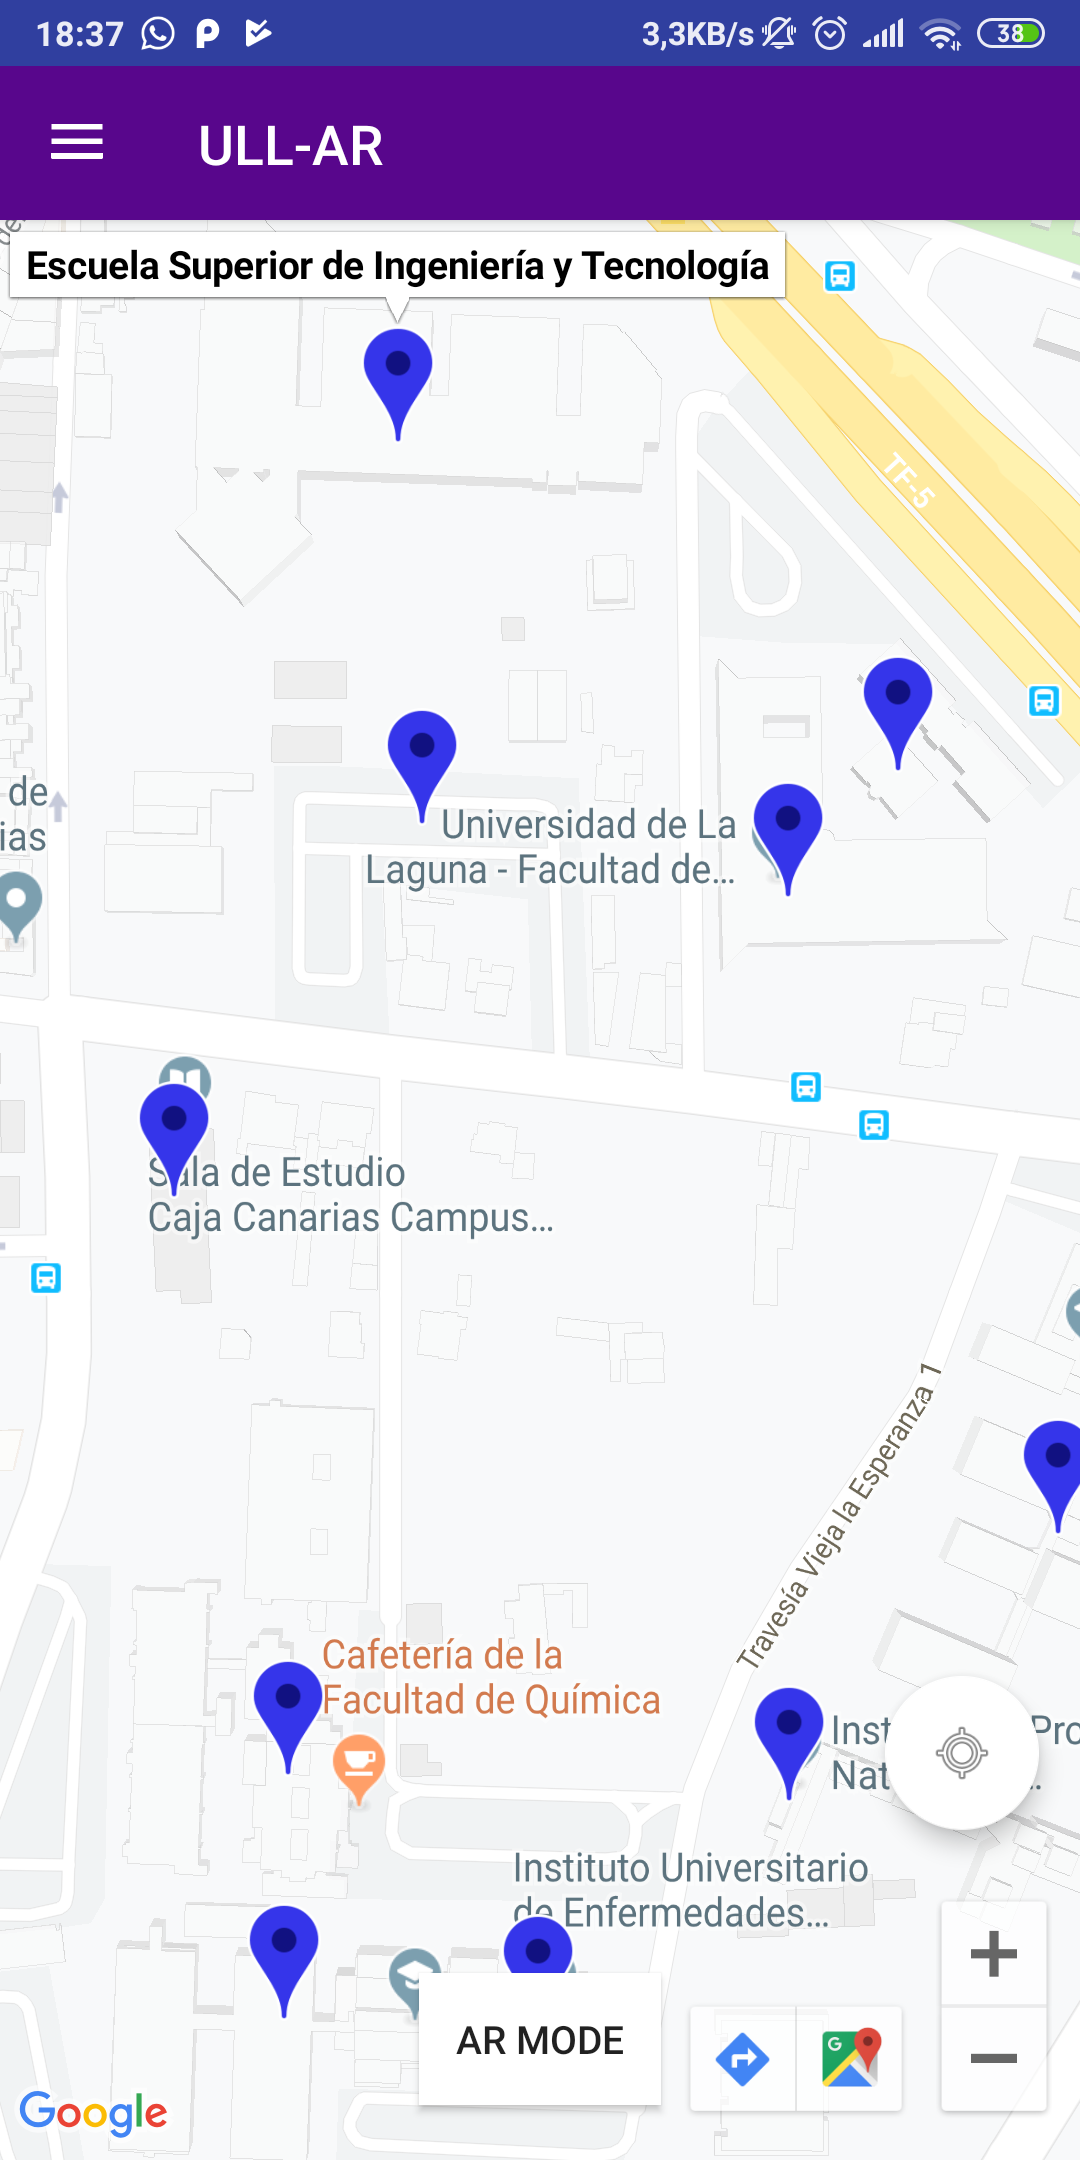
\includegraphics[width=0.7\linewidth]{Images/mapsApp}
			\end{center}
		\end{column}
	\end{columns}
\end{frame}


\begin{frame}
	\frametitle{\texttt{MapsFragment.java}}
	\lstinputlisting{Code/mapsfragment.java}
\end{frame}



% \begin{frame}
% 	\frametitle{\texttt{fragment\_maps.xml}}
% 	\lstinputlisting{Code/fragmentmaps.xml}
% \end{frame}

\begin{frame}
	\frametitle{Fragmentos de \ULLAR{}}
	\begin{columns}
		\begin{column}{0.6\textwidth}
			\block{HomeFragment}
			\begin{itemize}
				\item Primera vista que aparece cuando el usuario se autentifica en la aplicación.
				\item Uso del modelo de ``RecyclerView'' y adaptadores de Android.
				\item La clase ``ItemHome'' contiene los atributos a mostrar.
			\end{itemize}
			\endblock{}
		\end{column}
		\begin{column}{0.4\textwidth} 
			\vfill 
			\begin{center}
				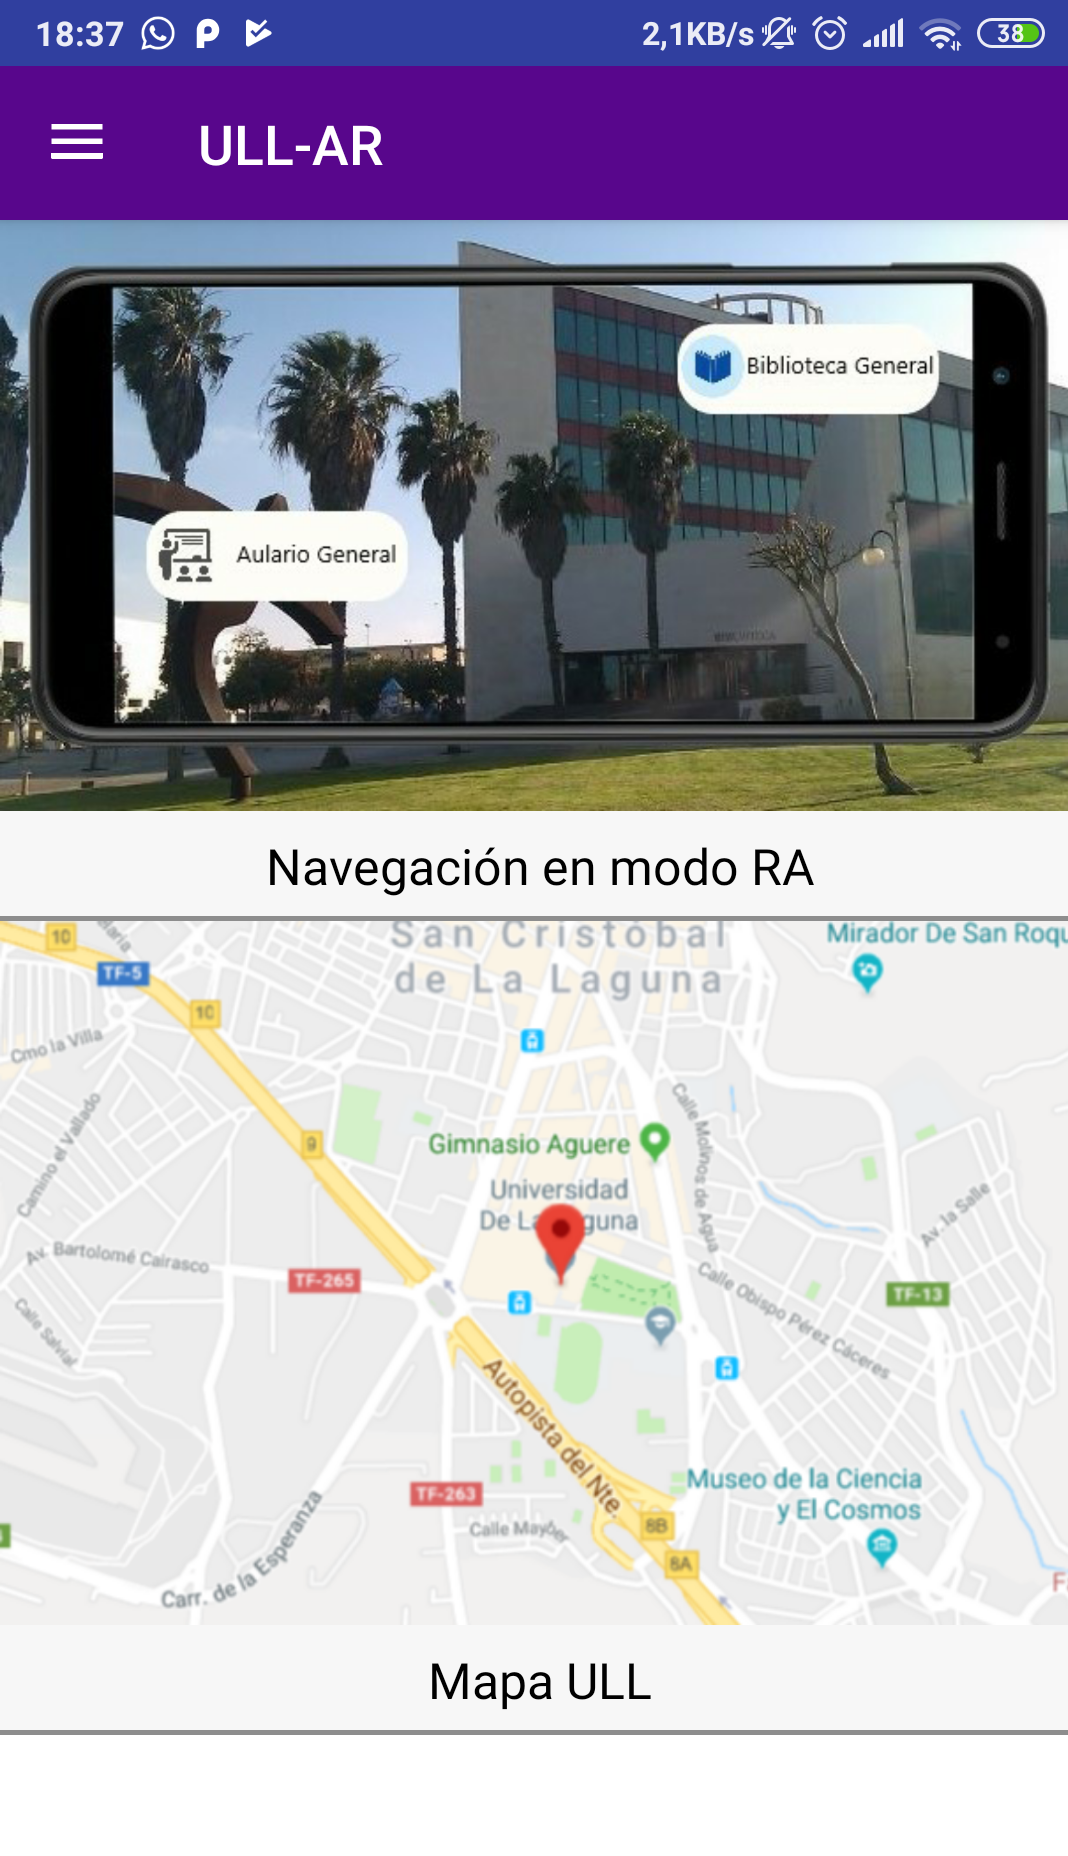
\includegraphics[width=0.8\linewidth]{Images/homeApp}
			\end{center}
		\end{column}
	\end{columns}
\end{frame}

         
      
\begin{frame}
	\frametitle{\texttt{ItemHomeAdapter.java}}
	\lstinputlisting{Code/homefragment1.java}
\end{frame}

         

\begin{frame}
	\frametitle{\texttt{HomeFragment.java}}
	\lstinputlisting{Code/homefragment2.java}
\end{frame}

\begin{frame}
	\frametitle{\texttt{fragment\_home.xml}}
	\lstinputlisting{Code/homefragment3.xml}
\end{frame}


\begin{frame}
	\frametitle{Fragmentos de \ULLAR{}}
	\begin{columns}
		\begin{column}{0.6\textwidth}
			\block{AboutFragment}
			\begin{itemize}
				\item Información general de la aplicación:
				\begin{itemize}
					\item Nombre.
					\item Autor.
					\item Version.
					\item Email.
					\item Descripción de la aplicación.
				\end{itemize}
			\end{itemize}
			\endblock{}
		\end{column}
		\begin{column}{0.4\textwidth} 
			\vfill 
			\begin{center}
				
\includegraphics[width=0.8\linewidth]{Images/infoApp}
			\end{center}
		\end{column}
	\end{columns}
\end{frame}


% \begin{frame}
% 	\frametitle{Menú de \ULLAR{}}
% 	\begin{columns}
% 		\begin{column}{0.6\textwidth}
% 			\block{Navigation Drawer}
% 			\begin{itemize}
% 				\item ¿Qué es un menú Navigation Drawer?.
% 				\item Se encuentra en multitud de aplicaciones.
% 				\item Mejor apariencia.
% 				\item Velocidad de carga entre fragmentos.
% 				\item La clase ``BaseActivity.java'' incorpora esté menú.
% 			\end{itemize}
% 			\endblock{}
% 		\end{column}
% 		\begin{column}{0.4\textwidth} 
% 			\vfill 
% 			\begin{center}
% 				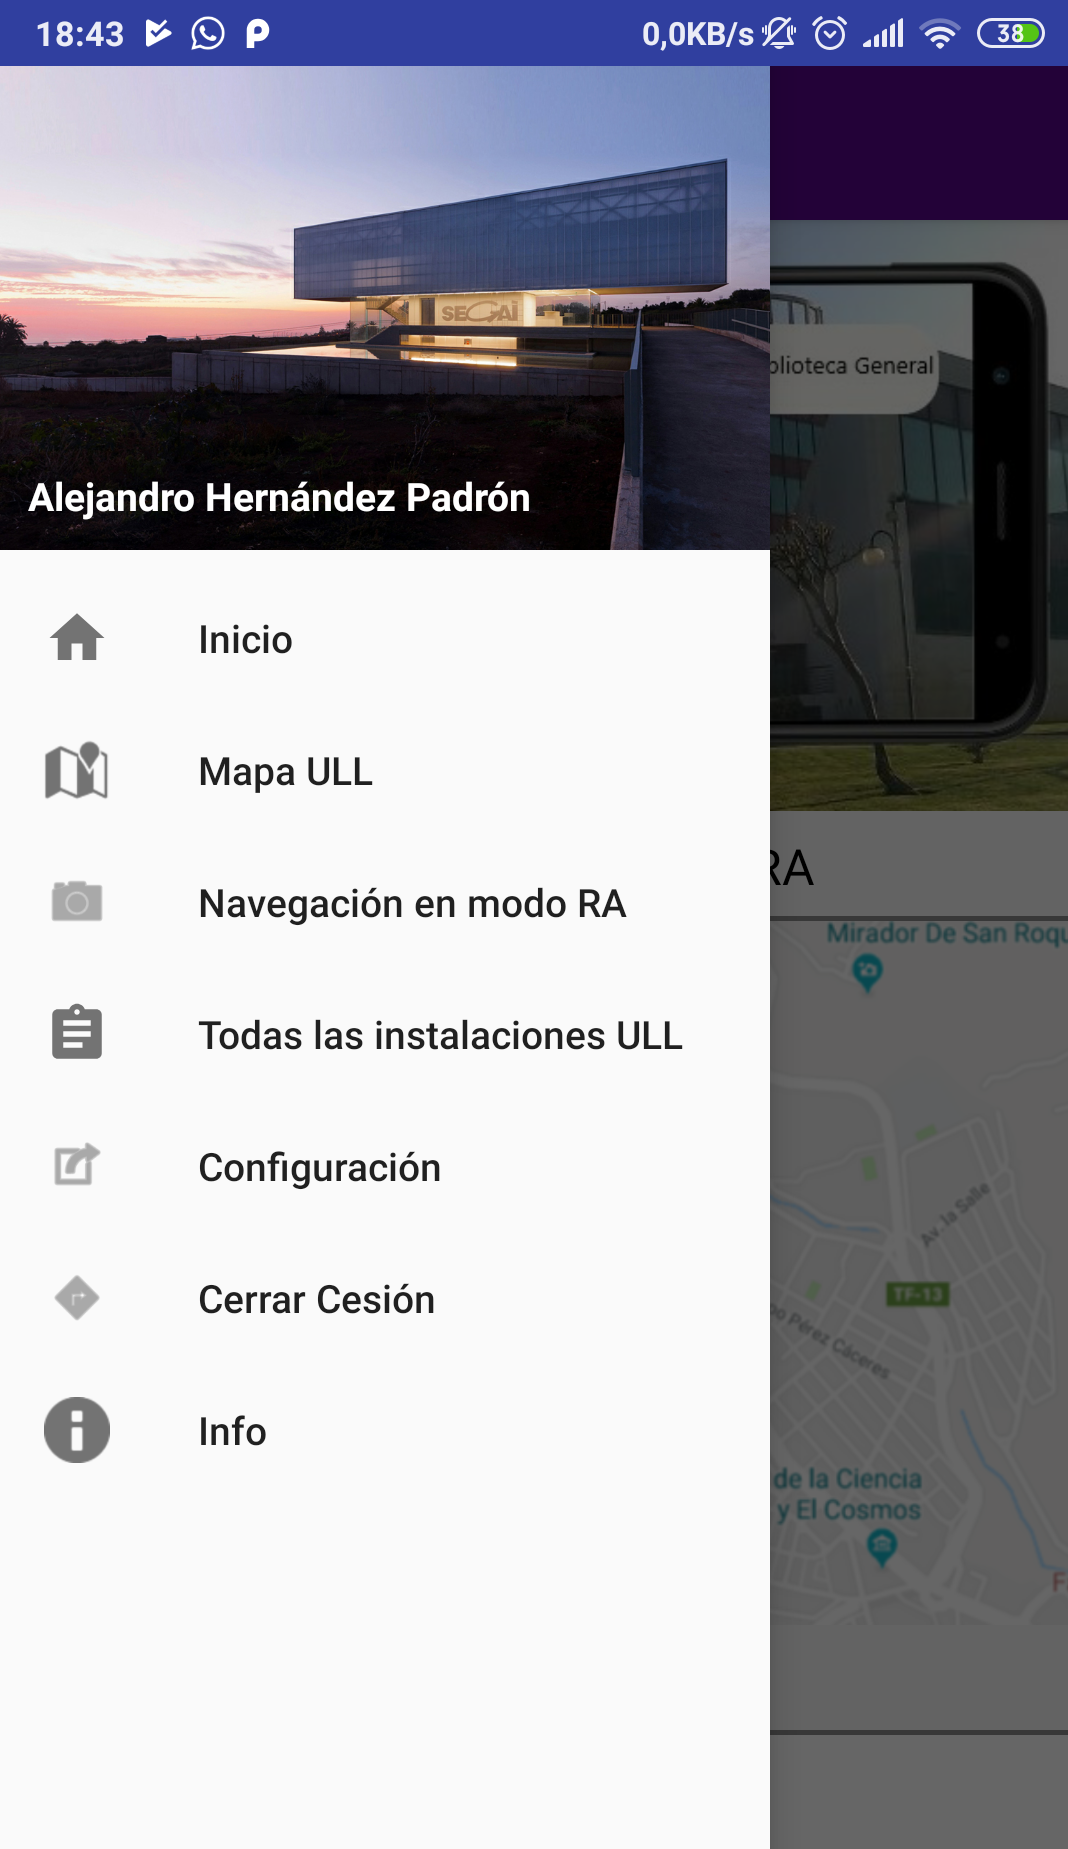
\includegraphics[width=0.8\linewidth]{Images/menuApp}
% 			\end{center}
% 		\end{column}
% 	\end{columns}
% \end{frame}



% \begin{frame}
% 	\frametitle{\texttt{navigation\_draw.xml}}
% 	\lstinputlisting{Code/menu1.xml}
% \end{frame}


% \begin{frame}
% 	\frametitle{\texttt{nav\_options.xml}}
% 	\lstinputlisting{Code/menu2.xml}
% \end{frame} 
 

% \begin{frame}
% 	\frametitle{\texttt{BaseActivity.java}}
% 	\lstinputlisting{Code/menu3.java}
% \end{frame} 
 
 

\begin{frame}
	\frametitle{Instalaciones de la ULL}
	\begin{columns}
		\begin{column}{0.6\textwidth}
			\block{Ventana de \textit{Todas las instalaciones}}
			\begin{itemize}
				\item Permite al usuario acceder a las instalaciones de la BD.
				\item Realizar una busqueda.
				\item Uso de adaptadores para mostrar información básica de cada instalación.
				\item Permite acceder a la ficha de información de cada instalación.
			\end{itemize}
			\endblock{}
		\end{column}
		\begin{column}{0.4\textwidth} 
			\vfill 
			\begin{center}
				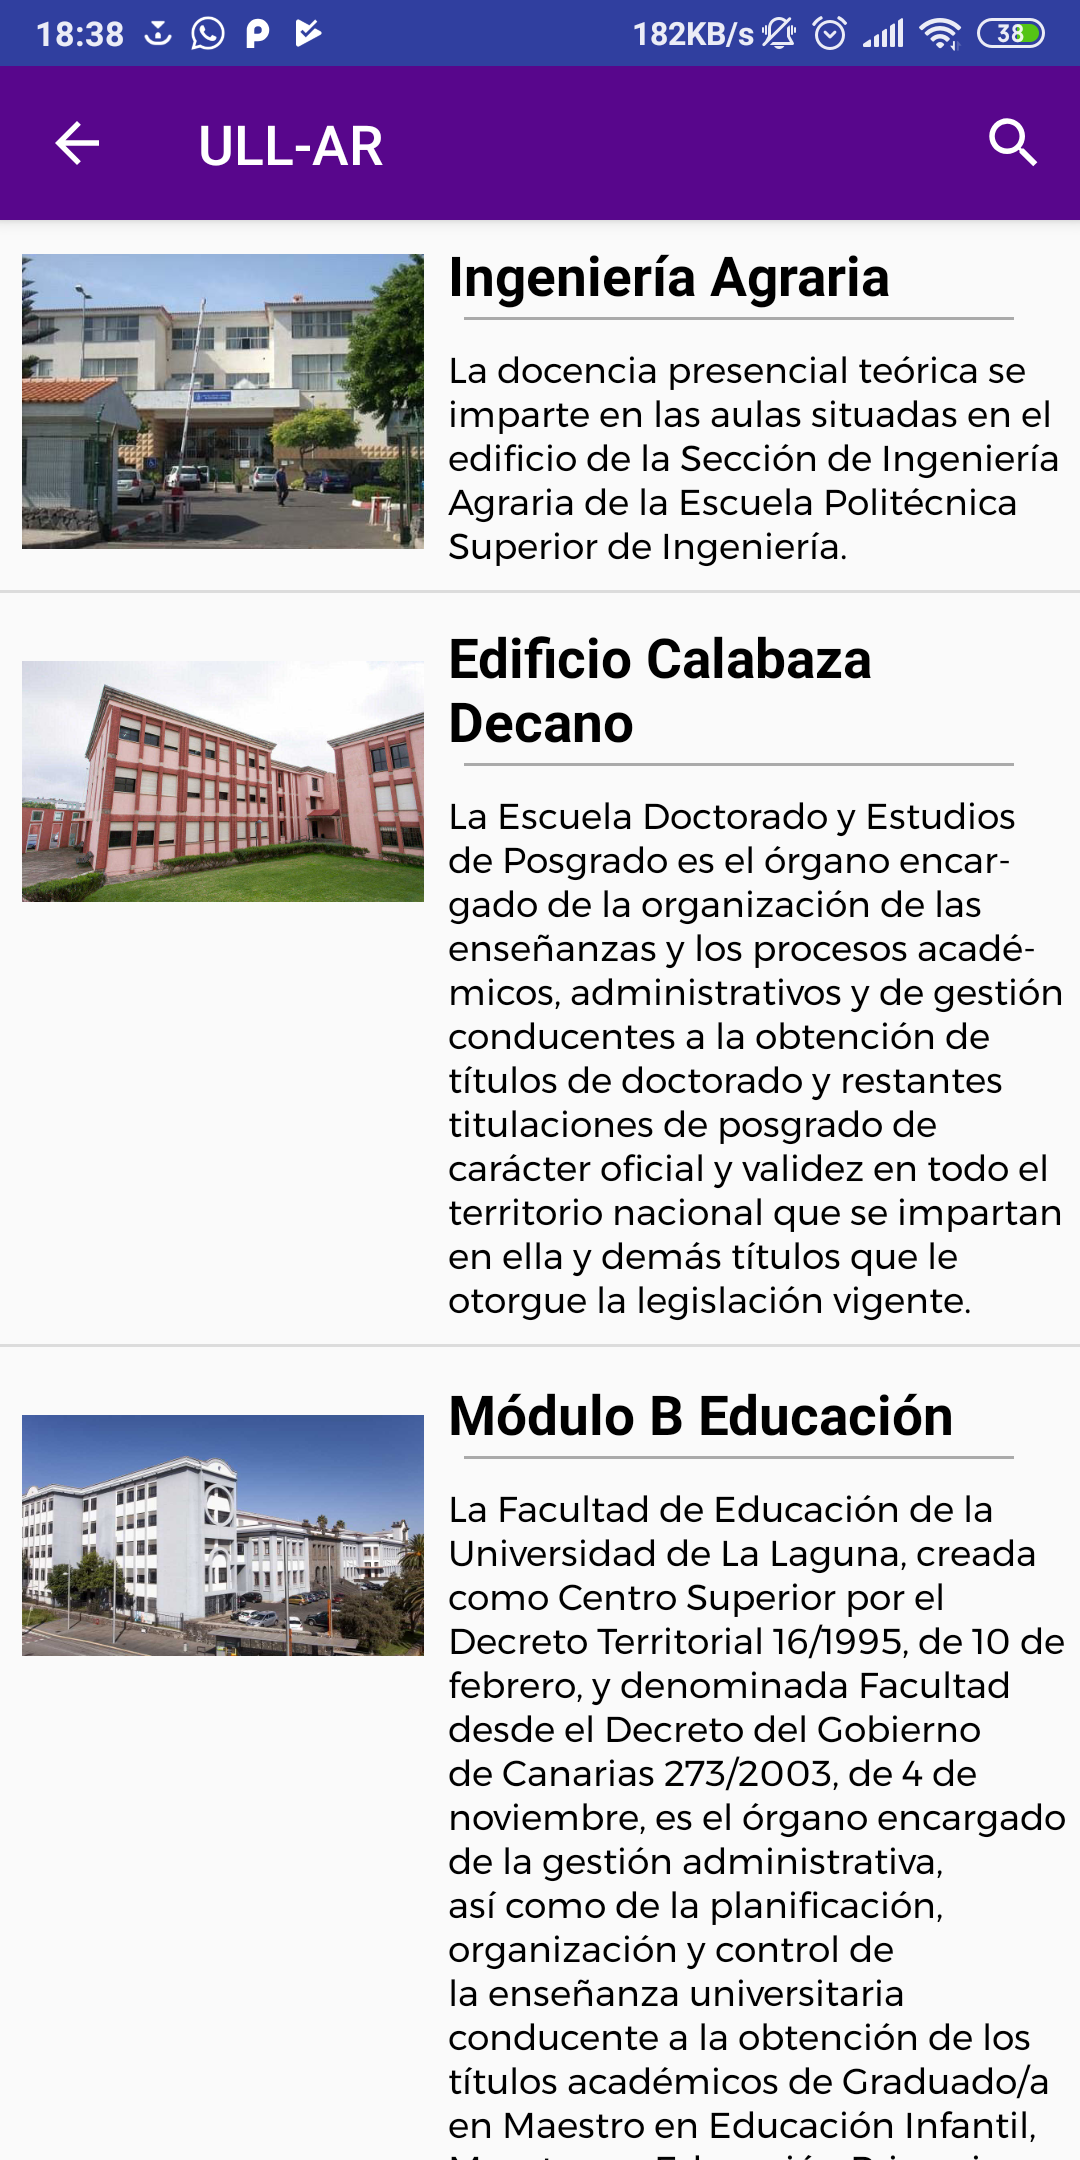
\includegraphics[width=0.75\linewidth]{Images/allSitesApp}
			\end{center}
		\end{column}
	\end{columns}
\end{frame} 
  

\begin{frame}
	\frametitle{\texttt{SiteAdapter.java}}
	\lstinputlisting{Code/instalaciones1.java}
\end{frame} 
 

\begin{frame}
	\frametitle{\texttt{SitesListActivity.java}}
	\lstinputlisting{Code/instalaciones2.java}
\end{frame}  

\begin{frame}
	\frametitle{\texttt{SitesListActivity.java}}
	\lstinputlisting{Code/instalaciones3.java}
\end{frame}  


\begin{frame}
	\frametitle{Instalaciones de la ULL}
	\begin{columns}
		\begin{column}{0.6\textwidth}
			\block{Ventana de \textit{Información de la instalación}}
			\begin{itemize}
				\item Muestra información detallada de la instalación.
				\item Permite acceder a la ruta a de la instalación en Google Maps.
				\item Muestra los enlaces de interes relacionados.
			\end{itemize}
			\endblock{}
		\end{column}
		\begin{column}{0.4\textwidth} 
			\vfill 
			\begin{center}
				
\includegraphics[width=0.75\linewidth]{Images/siteInfoApp}
			\end{center}
		\end{column}
	\end{columns}
\end{frame} 
  
\begin{frame}
	\frametitle{\texttt{SiteDescriptionActivity.java}}
	\lstinputlisting{Code/instalaciones4.java}
\end{frame}  


\begin{frame}
	\frametitle{Preferencias del usuario}
	\begin{columns}
		\begin{column}{0.6\textwidth}
			\block{Ventana de \textit{Información de la instalación}}
			\begin{itemize}
				\item Ventana donde van los ajustes de la aplicación
				\item Se pueden configurar los radios de busqueda de las instalaciones.
			\end{itemize}
			\endblock{}
		\end{column}
		\begin{column}{0.4\textwidth} 
			\vfill 
			\begin{center}
				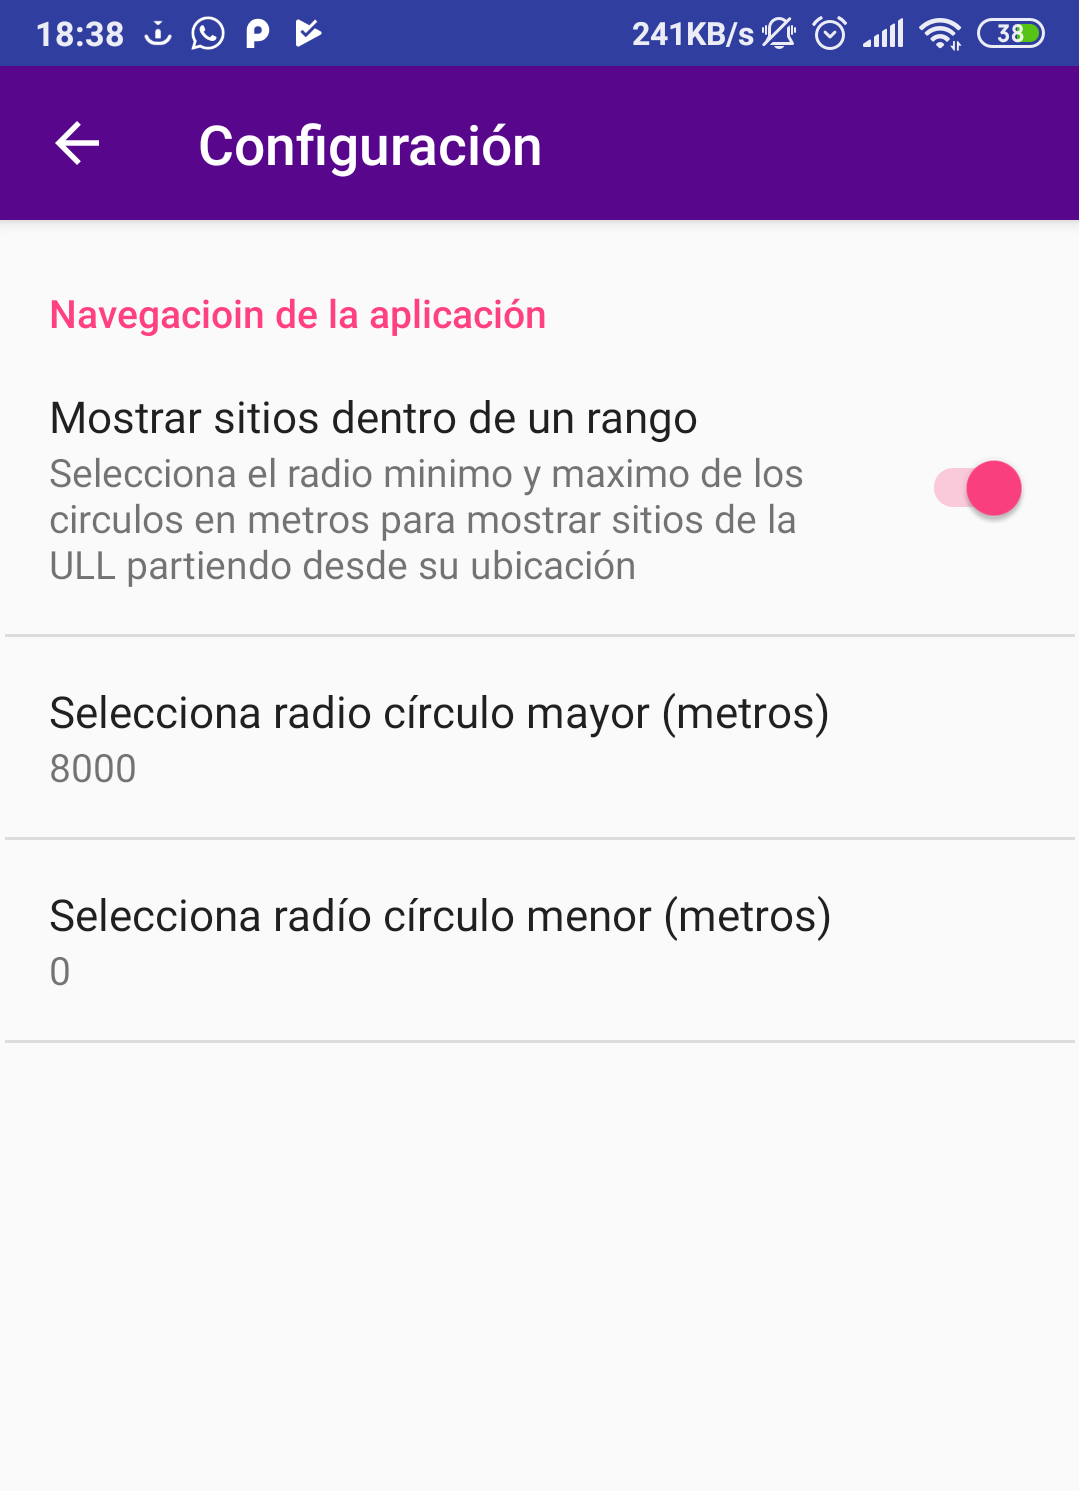
\includegraphics[width=0.9\linewidth]{Images/settingsApp}
			\end{center}
		\end{column}
	\end{columns}
\end{frame} 

% \begin{frame}
% 	\frametitle{\texttt{SiteAdapter.xml}}
% 	\lstinputlisting{Code/settings.xml}
% \end{frame}  
%----------------- ---------------------------------------------------

		\section{Despliegue}
			\begin{frame}
  \frametitle{Despliegue}
  \block{Repositorio de la aplicación}
    \begin{itemize}
		\item La aplicación ha sido almacenada en el repositorio GitHub como parte del PATFL.
    \item Se encuentra en GitHub: https://github.com/ccetsii/BulletPoint 
    \end{itemize}
  \endblock{}
\end{frame}
		\section{Presupuesto}	
			\begin{frame}
	\frametitle{Presupuesto}
	\block{Coste de los dispositivos}
		\begin{itemize}
			\item Autobuses: inversión de 500 euros y cubriríamos 20 paradas de autobús.
			\item Eventos: Para las 10 zonas de eventos se invertirían 250 euros.
			\item Aparcamientos: 8 aparcamientos. Mínimo 3 beacons por recinto. Desembolso de 600 euros.
			\item Asistencia y guía: cubriendo todos los edificios de la ULL se necesitarían unos 100 beacons, el importe asciende a 2500 euros.
			\item Total: 154 dispositivos con un coste de 3.850 euros.
		\end{itemize}
	\endblock{}
\end{frame}


\begin{frame}
	\frametitle{Presupuesto}
	\block{Despliegue de los dispositivos}
		\begin{itemize}
			\item Tarifa: 12,40 euros por hora trabajada.
			\item Se necesitaran 2 especialistas trabajando durante un mes a jornada completa (8 horas). 
			\item Total: 3.968 euros.
		\end{itemize}
	\endblock{}
\end{frame}


\begin{frame}
	\frametitle{Presupuesto}
	\block{Servidor para el almacenamiento de información}
		\begin{enumerate}
			\item Compra del servidor dedicado junto con el soporte y configuración servidor (cuota anual) : 1300 + 250 = 1.550 euros.
			\item Configuración de un servidor ya disponible en la Universidad (sin cuota anual de soporte ni mantenimiento): 550 euros.
		\end{enumerate}
	\endblock{}
\end{frame}


\begin{frame}
	\frametitle{Presupuesto}
	\block{Mantenimiento de la aplicación}
		\begin{itemize}
			\item Ofrecemos un especialista programador en Android.
			\item Este mantenimiento no incluye nuevas funcionalidades.
			\item Tarifa: 21.600 euros anuales netos durante el primer año y a 18.000 euros en adelante.
		\end{itemize}
	\endblock{}
\end{frame}
		\section{Summary and conclusions}
			\begin{frame} [fragile]
	\frametitle{Summary and conclusions}
	\block{Conclusions}
		Nowadays, beacon technology is still on a development stage.By itself can be quite limited due to the way it works.The physical and positional limitations require a deep analysis in order to place devices the best way.
		
		\bigskip
		On the other hand, each specific beacon provider tries to use his own SDKs to develop the applications.
		
		\bigskip
		The solution to this problem, in this case, has been found on the AltBeaconlibrary, which tries to bring close to developers this technology.
		
		\bigskip
	The achievement of this Final Year Project is to show that, many apps able to work with this technology exist or can be developed.
	
		\bigskip
		For now, we will keep on testing this technology and watching it grow.

	\endblock{}
\end{frame}
		\begin{frame}
  \frametitle{Agradecimientos}
  \block{Agradecimientos}
    \begin{itemize}
    \item Francisco de Sande González
		\item Familia y amigos.
    \end{itemize}
  \endblock{}
\end{frame}
		\include{Capitulos/Cap9_final}
%%%%%%%%%%%%%%%%%%%%%%%%%%%%%%%%%%%%%%%%%%%%%%%%%%%%%%%%%%%%%%%%%%%%%%%%%%%%%%%%%%%%%%%%%%%%
\end{document}